\htwo{Optical Character Recognition}
\label{sec:ocr}
\sectionauthor{Julian Kusternigg}

\hthree{Allgemeines}

"Optical Character Recognition", kurz OCR, ist eine Technik, um aus Bildern oder anderen Dokumentformaten (\zb: PDF) Zeichen herauszulesen und in Text umzuwandeln. Diesen Text kann der Computer dann für weitere Anwendungen verwenden. Dabei ist es egal ob der Text im Bild in Druckschrift oder Handschrift geschrieben ist. Ein Computer soll jeden Text, unabhängig der Schriftart, erkennen.
\cite{OCRIntro}

\hfour{Anwendung}

Schon 1914 wurden erste Schritte gemacht, um Zeichen einzulesen. Das "Optophone" ist ein Gerät, welches eingelesene Zeichen in Töne umwandelt. \cite{OCRRecognition}

1974 forschte Ray Kurzweil an einer OCR Technik, die jeden gedruckten Text, unabhängig der Schriftart, erkannte. Kurzweil entwickelte eine Maschine für Blinde und Menschen die nicht lesen konnten, indem der eingelesene Text von der Maschine vorgelesen wurde. \cite{OCRRecognition}

Heutzutage gibt es viele Anwendungen für die OCR Technologie. Zum Beispiel wird diese verwendet beim Projekt Gutenberg, eine der ältesten Digitalbibliotheken, um Bücher automatisch digitalisieren zu lassen. Aber auch im normalen Alltag stößt man öfters auf Texterkennung. So bietet zum Beispiel Google, bei ihrem Übersetzer, die Möglichkeit in Echtzeit über die Smartphone-Kamera Texte übersetzten zu lassen. Auch zum Einlesen von Informationen \zb: von einem Reisepass (wie bei "Lead Horizon"), wird Zeichenerkennung verwendet, um das mühsame Abschreiben zu vermeiden.

\hfour{Funktionalität}

Bevor man Texte aus einem Bild auslesen kann, wird das Bild meist vereinfacht. Es wird dabei das gesamte Bild auf Grautöne komprimiert, welche helfen sollen Text oder kein Text zu erkennen. Oft wird auch probiert das Bild zusammenzuschneiden, sodass nur mehr der wichtigste Teil mit Text vorhanden ist. Der letzte Schritt der gemacht wird ist das Einteilen der Zeichen. Dabei wird probiert alles was ein Zeichen sein könnte zu finden und auszuschneiden. \cite{OCRPreProcessing}

Diese Bildausschnitte von Zeichen werden dann probiert in den jeweiligen Zeichencode umgewandelt zu werden. Dafür gibt es zwei Herangehensweisen, um diese Umwandlung durchzuführen:

\begin{itemize}
    \item "Matrix Matching" oder auch "Pattern Matching" genannt
    \item "Feature Extraction"
\end{itemize}

\hfour{Matrix/Pattern Matching}

Bei diesem Vorgang wird eines der zusammengeschnittenen Zeichenbilder Pixel für Pixel verglichen, mit vorgefertigten Zeichen. Anhand der Prozent die übereinstimmen, kann zurückgeschlossen werden welches Zeichen im Bild sein könnte. Diese Möglichkeit ist recht einfach im Vergleich zur zweiten Technik. Ein Nachteil ist aber, dass verschiedene Schriftarten problematisch sein könnten und manche Zeichen falsch oder gar nicht erkannt werden. Beheben kann man dieses Problem, indem man die vorgefertigten Zeichen mit denen verglichen wird, erweitert. Das macht den ganzen Vorgang aber wiederum langsamer. Somit muss das Vorgehen für jede Anwendung individuell angepasst werden. \cite{OCRRecognition}

\hfour{Feature Extraction}

Hier wird, wie der Name schon sagt, nach Merkmalen gesucht. Merkmale sind zum Beispiel Kanten und Kurven. Diese braucht man, um Zeichen zu beschreiben. Die Merkmale werden dann mit einer Ansammlung von typischen Zeichenmerkmalen verglichen. Somit kann erkannt werden um welches Symbol es sich handeln könnte. Dieser Vorgang funktioniert oft besser mit verschieden Schriftarten, da nicht so wie bei Matrix Matching auf einen exakten Vergleich geschaut wird. \cite{OCRRecognition}

\hfour{Anwendung in der Praxis}

Heutzutage werden auch oft andere Ansätze verwendet. So extrahieren viele OCR Anbieter zuerst Merkmale von den Zeichen mit Bildern und ein neurales Netz prüft dann welches Zeichen das sein könnte.

Oft wird auch nicht nur nach Zeichen gesucht. Gerade bei Sprachen, die Wörter mit Leerzeichen trennen, versuchen OCR Anbieter diese komplett zu erfassen. Diese werden dann wieder in Zeichen zerlegt, aber trotzdem als gesamtes Wort mit einem Wörterbuch verglichen. Dadurch ist es noch wahrscheinlicher die Wörter richtig zu erkennen. 

\hfour{Tesseract}\label{sec:tesseract}

Tesseract ist eine Software-Bibliothek aus 1985, die 2005 als Open-Source-Projekt veröffentlicht wurde. Seit 2006 wird das Projekt von Google unterstützt und gilt als eine der bekanntesten "Optical-Character-Recognition" Bibliotheken. Zusätzlich zu den oben genannten Arten der Zeichenerkennung, verwendet Tesseract ein neurales Netz, um die Auswahl der Zeichen weiter einzuschließen. Außerdem probiert Tesseract ganze Wörter zu finden, die sich aus den Zeichen ergeben könnten, um noch genauere Ergebnisse zu liefern. \cite{Tesseract}

\hthree{Implementierung}

\hfour{OCR-Modul}
\label{sec:ocrmodul}

Man kann Raumnummern, nicht nur manuell eingeben, sondern auch mit der Kamera eines Smartphones einscannen. Für den Prozess, die Raumnummern aus den Bildern auszulesen, wird ein "Optical Character Recognition"-Verfahren verwendet. Dafür wird die Bibliothek "TesseractJS", eine Web-Version von "Tesseract OCR", direkt im Browser eingebunden. \cite{TesseractJS}\cite{TesseractJSImplementation}

Für diese Aufgabe gibt es bei \ZELIA\ im Komponentensystem eine Komponente. Diese Komponente wird auf der OCR-Seite des Frontends eingebunden. Sie beinhaltet ein Videoelement, um zu zeigen was sie scannt. Bevor die Kamera eines Gerätes für eine Webseite verwendet werden darf, muss über den "Browser Navigator" die Berechtigung auf den Kamerazugriff angefragt werden (siehe Code \ref{code:CameraAccess}).

\typescript[code:CameraAccess]{code/OCR/nav.ts}{Zugriff auf eine Kamera im Browser}

Als Parameter bei dieser Anfrage kann man definieren worauf man Zugriff haben möchte. Im Falle von \ZELIA\ wird als Videoquelle die Außenkamera angefragt. Audioaufnahmen werden verworfen, da sie nicht notwendig sind. Die Browser bestimmen dann, ob die Anfrage erlaubt werden soll oder fragen die Benutzer*innen des Gerätes. Wenn der Zugriff abgelehnt wird, wird das Videoelement, welches die Kamera anzeigt, durch eine Fehlermeldung ersetzt. Darf der Browser aber die Videoquelle verwenden, so zeigt er sie an und startet das "OCR"-Modul.

\begin{figure}[H]
    \centering
    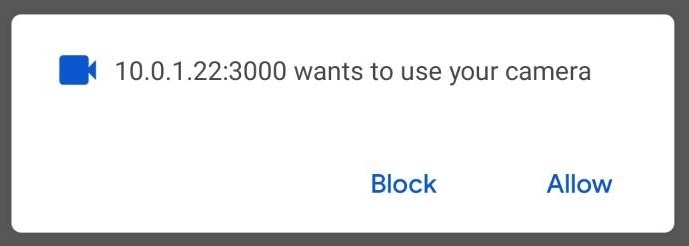
\includegraphics[width=120mm]{media/OCR/cam_access_light.jpg}
    \caption{Abfragen des Kamerazugriffs}
\end{figure}


Die Aufgabe des "OCR"-Moduls ist es Bilder in Text umzuwandeln. Dabei wird TesseractJS verwendet, um den "Optical Character Recognition" Prozess durchzuführen. TesseractJS ist eine einfach verwendbare Bibliothek, die zum Testen von OCR bei \ZELIA\ verwendet wurde. Da diese Tests gute Ergebnisse geliefert haben, wurde die Einsatzweise optimiert und weiterverwendet.

\typescript{code/OCR/OCRModule.ts}{Die Verwendeung von TesseractJS}

TesseractJS verwendet sogenannte "Worker", um Text aus einem Bild zu extrahieren. Je mehr davon vorhanden sind, desto schneller geht der Prozess. Natürlich wird dadurch mehr Prozessorleitung verwendet, was bei Smartphones schnell zu einem erhöhten Energieverbrauch oder Erhitzen des Gerätes führt. Somit wird bei \ZELIA\ standardmäßig nur ein "Worker" verwendet. Da das Initialisieren dieser Services recht lange dauert, ca. 2-3 Sekunden, gäbe es die Möglichkeit mehrere "Worker" gleichzeitig zu laden. Dadurch kann viel Zeit beim Initialisieren eingespart werden. Bei nur einem "Worker" gibt es diesen Unterschied nicht. 

Zusätzlich, um den eigentlichen Umwandlungsvorgang von Bild zu Text zu beschleunigen, wird eine Bildoptimierung für OCR durchgeführt. Bevor Tesseract dem Bild die Zeichen entzieht, wird es in ein Schwarz-Weiß-Bild umgewandelt und auf den wichtigen Teil, dort wo nichts schwarz ist, zusammengeschnitten (siehe Abbildung \ref{ocroptimised}).

Nachdem das Bild vereinfacht wurde, wird der eigentliche OCR Prozess durchgeführt. Im besten Fall kommt nur die gewünschte Raumnummer als Ergebnis heraus. In der Realität werden aber auch andere Zeichen wie Beistriche, Rufzeichen und manchmal, bei schlecht beleuchteten Bildern, sogar Buchstaben gefunden, die eigentlich gar nicht vorhanden sein sollten. Das ist im Fall von \ZELIA\ allerdings kein so großes Problem, denn alle Raumnummern sind gleich aufgebaut. Somit wird mit "Regular Expressions" ("{\ttfamily [A-Z]?[0-9]\{4\}(\textbackslash.[0-9])?\$}") der gesuchte Teil herausgefiltert und falls es eine Raumnummer gibt, wird geprüft, ob ein Raum mit dieser Nummer existiert.

Mit diesen Optimierungen liefert Tesseract sehr gute Ergebnisse, ein Grund weshalb bei \ZELIA\ die Open-Source Bibliothek verwendet wird.

\typescript{code/OCR/compress.ts}{Bild vereinfachen, bevor Text extrahiert wird}

\begin{figure}
    \centering
    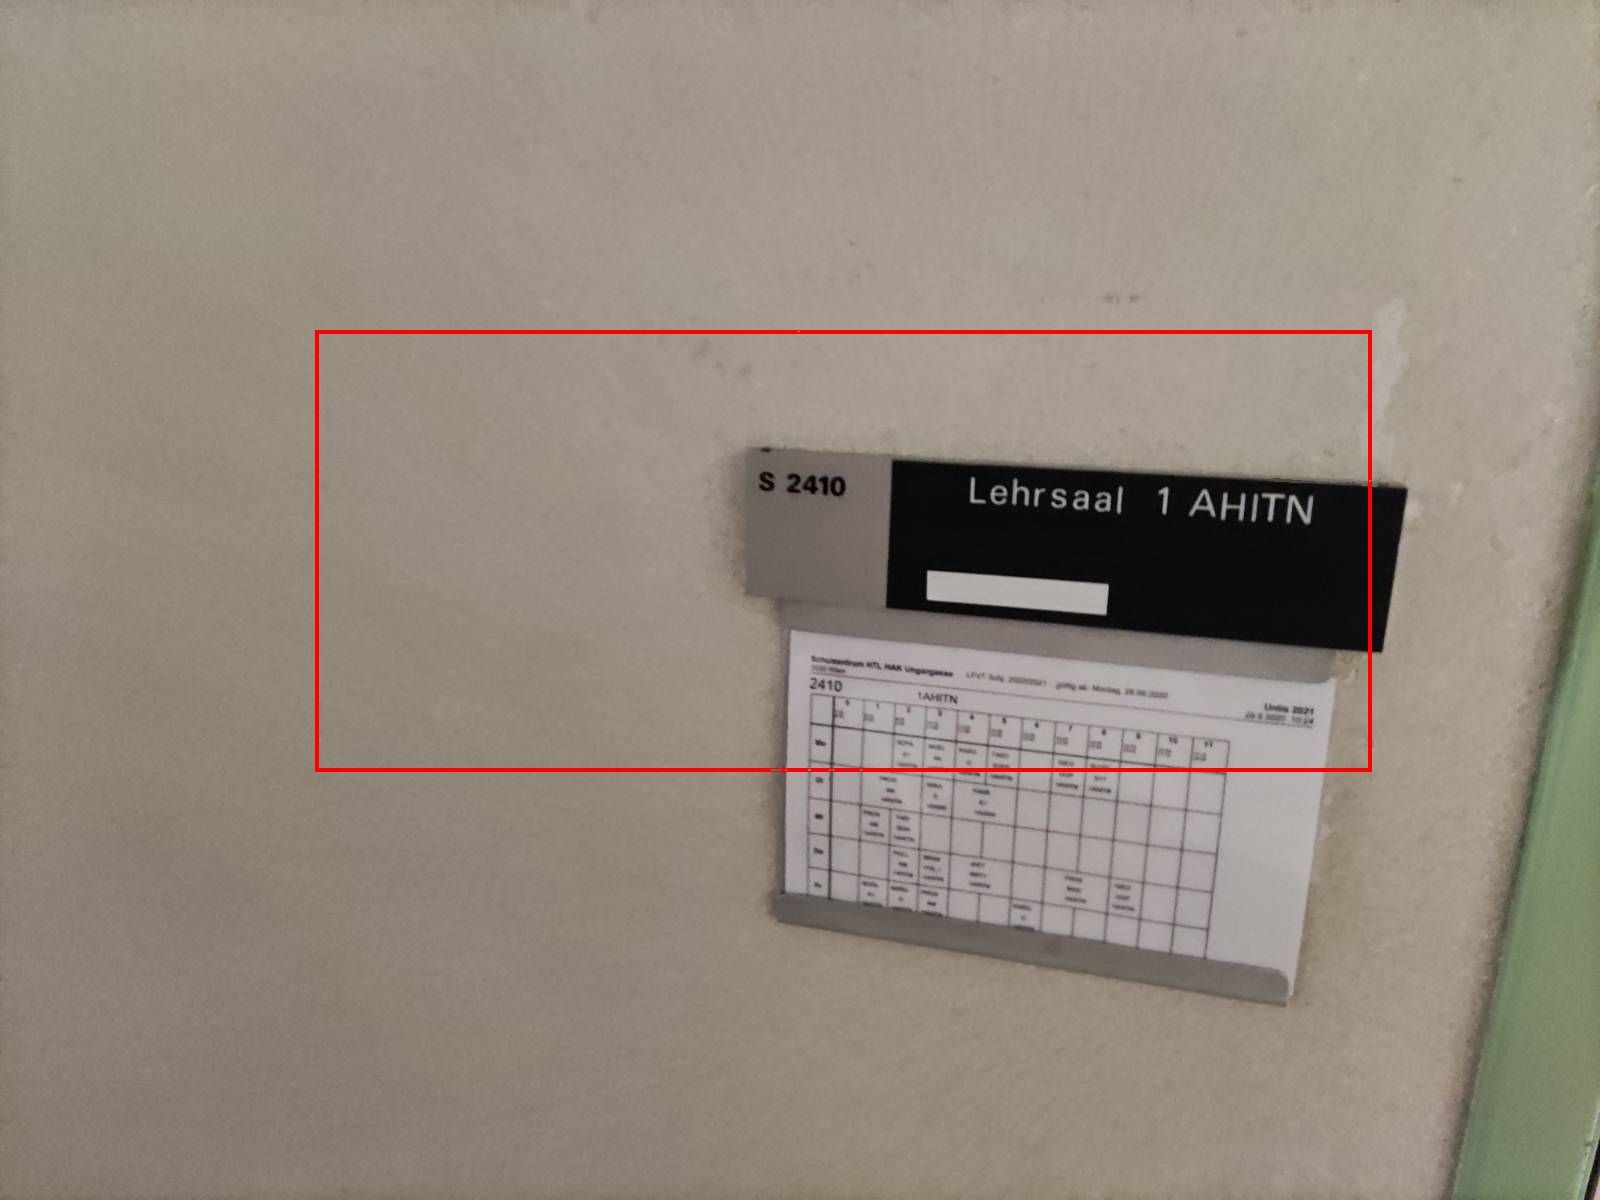
\includegraphics[width=120mm]{media/OCR/original}
    \caption{Aufnahme einer Smartphonekamera (Fokusbereich rot markiert)}
    \label{fig:phonecam}
\end{figure}


\begin{figure}
    \centering
    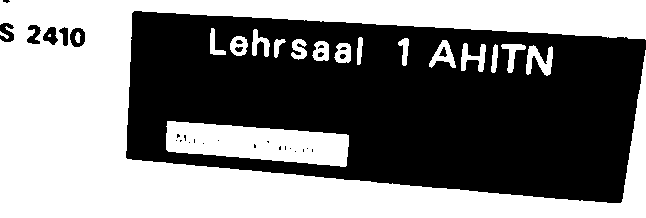
\includegraphics[width=120mm]{media/OCR/compressed}
    \caption{Bild, nachdem es für das OCR-Modul vereinfacht wurde}
    \label{ocroptimised}
\end{figure}

% TODO show result: S 2410   Lehrsaal 1 AHITN

\pagebreak

\hfour{Messungen der OCR Implementierung}
\label{sec:ocrmessung}

Um zu überprüfen ob das OCR-Modul für die Anwendung auf Mobilgeräten performant genug ist, wurden einige Messungen durchgeführt. Der OCR Umwandlungsprozess von dem Bild, welches in der Abbildung \ref{fig:phonecam} zu sehen ist, dauert ohne die Bildvereinfachung rund 4,2 Sekunden. Für die schnelle Anwendung bei \ZELIA\ wäre diese Dauer viel zu lange. Damit dieser Prozess verkürzt wird, ist ein Fokusbereich definiert, auf den das Bild verkleinert wird (siehe Abbildung \ref{fig:ocrfocus}). Durch diese Verkleinerung dauert der OCR-Vorgang nur noch rund 1,3 Sekunden. Dieses Ergebnis ist schon besser, wurde jedoch noch weiter optimiert, um die Dauer zu minimieren. 

\begin{figure}[H]
    \centering
    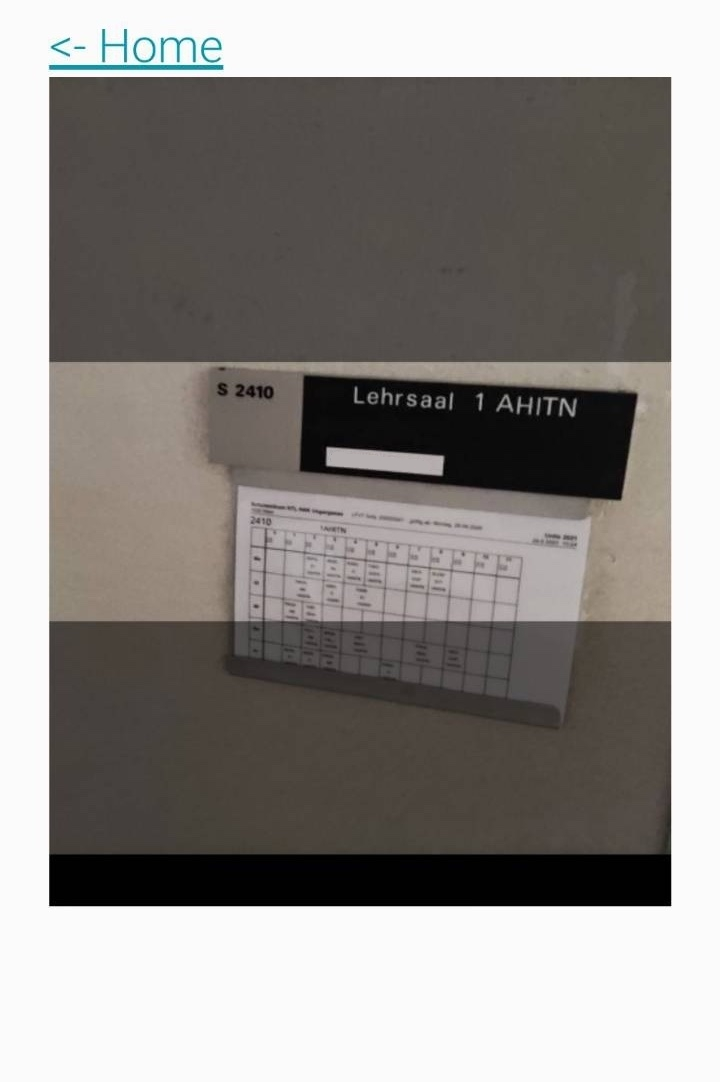
\includegraphics[width=80mm]{media/WebComponents/OCRSeite_light.jpg}
    \caption{OCR-Seite}
    \label{fig:ocrfocus}
\end{figure}

Wie oben geschrieben wandelt \ZELIA\ das Bild der Kamera in ein Schwarz-Weiß-Bild um und schneidet es so klein wie möglich zusammen, bevor es dem Tesseract Prozess übergeben wird. Diese Optimierung dauert rund 27 Millisekunden und beschleunigt den gesamten Prozess. Den Text aus dem oben genannten Bild zu extrahieren, dauert dadurch nur noch rund 660 Millisekunden. Das Bild in ein Schwarz-Weiß-Bild umzuwandeln, macht für Tesseract eigentlich kaum einen Unterschied. Trotzdem wird es so gemacht, weil das Verkleinern eines Bildes mit Hilfe der äußersten schwarzen Punkte funktioniert. Diese Verkleinerung, ist so wie der kleinere Fokusbereich, ausschlaggebend für schnelle Ergebnisse. 

Der letzte Optimierungsversuch war mehrere "Worker" zu verwenden. Mit diesem Ansatz hat man allerdings kaum Zeit gewonnen, da mehrere "Worker" erst richtig performant werden, wenn man große Mengen an Text aus Bildern filtern will. Während das Initialisieren von einem OCR "Worker" rund 2,3 Sekunden dauert, benötigen zwei Worker rund 3,4 Sekunden. Dadurch, dass bei \ZELIA\ die "Worker" wie oben genannt gleichzeitig geladen werden, wird dieser Vorgang beschleunigt. Trotzdem steigt die Dauer leicht an wenn mehrere "Worker" initialisiert werden. Wenn ein OCR Prozess mit zwei "Workern" das Bild aus dem vorherigen Beispiel verarbeitet, dauert dies rund 630 Millisekunden. Diese Optimierung, von rund 30 Millisekunden, wird durch die längere Startzeit der zwei "Worker", mit über einer Sekunde, aufgehoben.

Nochmal kurz zusammengefasst: Die durchschnittlichen Zeiten, die das OCR-Modul insgesamt braucht, liegen zwischen 400 und 700 Millisekunden, abhängig davon wie groß die Buchstaben in dem Fokusbereich stehen, also wie nahe die Kamera vom Schild entfernt ist.

